84. $f(x)=\begin{cases} \sqrt{1-x},\ \text{ если } x\leqslant0,\\
x^2-|2x+1|,\ \text{ если } x>0.\end{cases}=\begin{cases} \sqrt{1-x},\ \text{ если } x\leqslant0,\\
x^2-2x-1,\ \text{ если } x>0.\end{cases}$
$$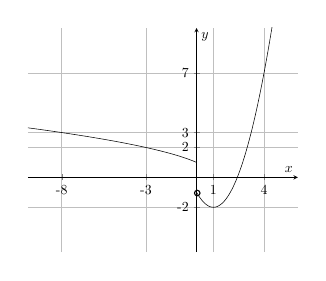
\begin{tikzpicture}[scale=0.5]
\begin{axis}[
    axis lines = middle,
    grid=major,
    legend pos={south west},
    xlabel = {$x$},
    %xlabel style={below right},
    ylabel = {$y$},
    ymin=-5,
    ymax=10,
    xmin=-10,
    xmax=6,
    xtick={-8, -3, 1, 4},
    xticklabels={-8, -3, 1, 4},
    ytick={-2,2, 3, 7},
    yticklabels={-2,2, 3, 7},
                  ]
	\addplot[domain=-10:0, samples=100, color=black] {sqrt(1-x)};
    \addplot[domain=0.01:10, samples=100, color=black] {x*x-2*x-1};
        %\addplot[domain=2.01:6, samples=100, color=black] {2/(2-x)};
   % \addplot[domain=-3:3, samples=100, color=black] {-x};
     %\addlegendentry{$\text{Рис. 1}$};
\end{axis}
\draw (4.3,1.5) circle (2pt);
%\draw (3.45,0.75) circle (2pt);
%\draw (3.45,2.55) circle (2pt);
\end{tikzpicture}$$
